
%(BEGIN_QUESTION)
% Copyright 2011, Tony R. Kuphaldt, released under the Creative Commons Attribution License (v 1.0)
% This means you may do almost anything with this work of mine, so long as you give me proper credit

Anta at den elektriske motoren nekter å gå når ``Run''-trykknappen trykkes.  En tekniker starter feilsøking av kretsen, i rekkefølgen vist under:

$$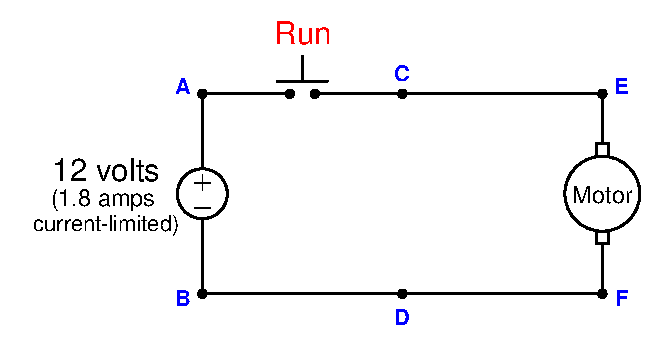
\includegraphics[width=15.5cm]{i00194x01.eps}$$

\begin{itemize}
\item{} {\bf Test 1:} Målt 2.8 ohm mellom punkt {\bf E} og {\bf F}, med ``Run''-bryter ikke trykket inn.
\vskip 25pt
\item{} {\bf Test 2:} Målt 12 volt mellom punkt {\bf A} og {\bf F}, med ``Run''-bryter ikke trykket inn.
\vskip 25pt
\item{} {\bf Test 3:} Målt 12 volt mellom punkt {\bf A} og {\bf B}, med ``Run''-bryter ikke trykket inn.
\vskip 25pt
\item{} {\bf Test 4:} Målt 12 volt mellom punkt {\bf A} og {\bf C}, med ``Run''-bryter trykket inn.
\vskip 25pt
\end{itemize}

Identifiser nyttig informasjon om type eller plassering av feilen ut fra resultatene av hver test, i samme rekkefølge som testene ble utført.  Hvis testen ikke er nyttig (dvs. ikke gir ny informasjon), marker den som det.  Anta at det bare er én feil i kretsen, og identifiser plassering og type feil så presist du kan fra testresultatene over.

\vfil 

\underbar{file i00194}
\eject
%(END_QUESTION)





%(BEGIN_ANSWER)

\begin{itemize}
\item{} {\bf Test 1:} Målt 2.8 ohm mellom punkt {\bf E} og {\bf F}, med ``Run''-bryter ikke trykket inn.  {\it Beviser at motoren ikke har brudd, og sannsynligvis heller ikke er kortsluttet.}
\vskip 5pt
\item{} {\bf Test 2:} Målt 12 volt mellom punkt {\bf A} og {\bf F}, med ``Run''-bryter ikke trykket inn.  {\it Beviser at kilden ikke er død, og at ledningene B-D-F er i orden.}
\vskip 5pt
\item{} {\bf Test 3:} Målt 12 volt mellom punkt {\bf A} og {\bf B}, med ``Run''-bryter ikke trykket inn.  {\it Unødvendig test, siden vi allerede vet at kilden ikke er død.}
\vskip 5pt
\item{} {\bf Test 4:} Målt 12 volt mellom punkt {\bf A} og {\bf C}, med ``Run''-bryter trykket inn.  {\it Beviser at bryteren har brudd, siden den skulle hatt 0 volt fall når den trykkes inn.}
\end{itemize}

\vskip 10pt

{\bf Feilen er en ``åpen'' trykknappbryter (brudd).}

%(END_ANSWER)





%(BEGIN_NOTES)


%INDEX% Troubleshooting review: electric circuit diagnostic test rationale

%(END_NOTES)

